\begin{figure}[h]
\centering
\begin{tikzpicture}
    \begin{customlegend}[legend columns=3,
        legend entries={{SkeTRAG (PageRank)},{(Graph$+$Text)RAG ($\theta=0.2$)}, {TextRAG}}
        ,
        legend style={at={(0.45,1.05)},anchor=north,draw=none,font=\footnotesize,column sep=0.1cm}]
    \addlegendimage{line width=0.3mm,mark size=2pt,mark=o,color=Red}
    \addlegendimage{line width=0.3mm,mark size=2pt,mark=pentagon,color=Green}
    \addlegendimage{line width=0.3mm,mark size=2pt,mark=triangle,color=LightBlue}
    \end{customlegend}
\end{tikzpicture}
\\[-\lineskip]
\subfloat[MuSiQue]{
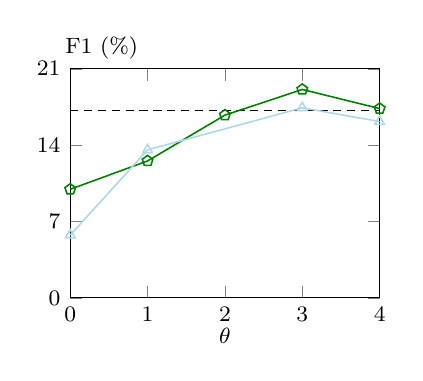
\begin{tikzpicture}[scale=1]
    \begin{axis}[
        height=\columnwidth/2.7,
        width=\columnwidth/2.2,
        ylabel={F1 (\%)},
        xlabel={$\theta$},
        xmin=0, xmax=4,
        ymin=0, ymax=0.21,
        xtick={0,1,2,3,4},
        xticklabel style = {font=\footnotesize},
        xticklabels={0,1,2,3,4},
        ytick={0, 0.07, 0.14, 0.21},
        yticklabels={0, 7, 14, 21},
        every axis y label/.style={at={(current axis.north west)},right=4mm,above=0mm},
        label style={font=\footnotesize},
        tick label style={font=\footnotesize},
        every axis x label/.style={at={(current axis.south)},right=0mm,above=-7mm},
        label style={font=\footnotesize},
        tick label style={font=\footnotesize},
    ]
\addplot[densely dashed, color=black, line width=0.1mm] coordinates {(0, 0.171508414) (4, 0.171508414)};
    \addplot[line width=0.2mm,mark size=2pt,mark=o,color=Red]
        plot coordinates { % SkeTRAG

    };

    \addplot[line width=0.2mm,mark size=2pt,mark=pentagon,color=Green]
        plot coordinates { % Hybrid
(0, 0.099545614)
(1, 0.125519636)
(2, 0.167524344)
(3, 0.191059656)
(4, 0.173562826)
    };

    \addplot[line width=0.2mm,mark size=2pt,mark=triangle,color=LightBlue]
        plot coordinates { % TextRAG
(0, 0.057530199)
(1, 0.135702597)
(3, 0.17426039)
(4, 0.161658265)
    };

    \addplot[line width=0.2mm,mark size=2pt,mark=x,color=DeepBlue]
        plot coordinates { % Skeleton

    };
    \end{axis}

\end{tikzpicture}

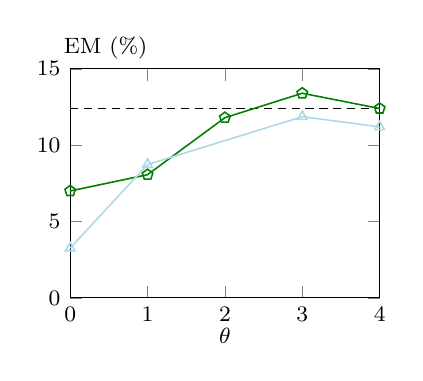
\begin{tikzpicture}[scale=1]
    \begin{axis}[
        height=\columnwidth/2.7,
        width=\columnwidth/2.2,
        ylabel={EM (\%)},
        xlabel={$\theta$},
        xmin=0, xmax=4,
        ymin=0.0, ymax=0.15,
        xtick={0,1,2,3,4},
        xticklabel style = {font=\footnotesize},
        xticklabels={0,1,2,3,4},
        ytick={0, 0.05, 0.10, 0.15},
        yticklabels={0, 5, 10, 15},
        every axis y label/.style={at={(current axis.north west)},right=4.5mm,above=0mm},
        label style={font=\footnotesize},
        tick label style={font=\footnotesize},
        every axis x label/.style={at={(current axis.south)},right=0mm,above=-7mm},
        label style={font=\footnotesize},
        tick label style={font=\footnotesize},
    ]

\addplot[densely dashed, color=black, line width=0.1mm] coordinates {(0, 0.124) (4, 0.124)};
    \addplot[line width=0.2mm,mark size=2pt,mark=o,color=Red]
        plot coordinates { % SkeTRAG

    };

    \addplot[line width=0.2mm,mark size=2pt,mark=pentagon,color=Green]
        plot coordinates { % Hybrid
(0, 0.07)
(1, 0.080666667)
(2, 0.118)
(3, 0.134)
(4, 0.124)
    };

    \addplot[line width=0.2mm,mark size=2pt,mark=triangle,color=LightBlue]
        plot coordinates { % TextRAG
(0, 0.032666667)
(1, 0.087333333)
(3, 0.118666667)
(4, 0.112)
    };
    
    \end{axis}

\end{tikzpicture}

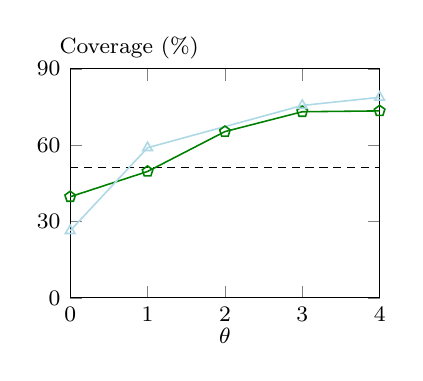
\begin{tikzpicture}[scale=1]
    \begin{axis}[
        height=\columnwidth/2.7,
        width=\columnwidth/2.2,
        ylabel={Coverage (\%)},
        xlabel={$\theta$},
        xmin=0, xmax=4,
        ymin=0.0, ymax=0.9,
        xtick={0,1,2,3,4},
        xticklabel style = {font=\footnotesize},
        xticklabels={0,1,2,3,4},
        ytick={0, 0.3, 0.6, 0.9},
        yticklabels={0, 30, 60, 90},
        every axis y label/.style={at={(current axis.north west)},right=7.5mm,above=0mm},
        label style={font=\footnotesize},
        tick label style={font=\footnotesize},
        every axis x label/.style={at={(current axis.south)},right=0mm,above=-7mm},
        label style={font=\footnotesize},
        tick label style={font=\footnotesize},
    ]

\addplot[densely dashed, color=black, line width=0.1mm] coordinates {(0, 0.514666667
) (4, 0.514666667
)};

    \addplot[line width=0.2mm,mark size=2pt,mark=o,color=Red]
        plot coordinates { % SkeTRAG

    };

    \addplot[line width=0.2mm,mark size=2pt,mark=pentagon,color=Green]
        plot coordinates { % Hybrid
(0, 0.397333333)
(1, 0.496666667)
(2, 0.653333333)
(3, 0.731333333)
(4, 0.734666667)

    };

    \addplot[line width=0.2mm,mark size=2pt,mark=triangle,color=LightBlue]
        plot coordinates { % TextRAG
(0, 0.264)
(1, 0.59)
(3, 0.756)
(4, 0.788)
    };
    
    \end{axis}

\end{tikzpicture}
}%
\caption{Answer quality of PageRank sampling algorithms by varying \#chunk bisections. Dash line represents the performance of GraphRAG.} \label{fig:quality-chunk}
\end{figure}